\documentclass[11pt,a4paper,titlepage]{article}
\usepackage[utf8]{inputenc}
\usepackage{amsmath}
\usepackage{amsfonts}
\usepackage{braket}
\usepackage{csvsimple}
\usepackage{amssymb}
\usepackage{subcaption}
\usepackage{hyperref}
\hypersetup{
    colorlinks=true,
    linkcolor=black,
    filecolor=black,
    urlcolor=cyan,
    citecolor=black,
}
\usepackage{tikz}
\usetikzlibrary{calc,patterns,angles,quotes,shapes.geometric, arrows}

\def\layersep{2.5cm}
\def\layersepSmall{1.2cm}

\tikzstyle{train} = [rectangle, rounded corners, minimum width=2.2cm, minimum height=1cm,text centered, draw=black, fill=red!30]
\tikzstyle{test} = [rectangle, rounded corners, minimum width=2.2cm, minimum height=1cm,text centered, draw=black, fill=green!30]
\tikzstyle{data} = [rectangle, rounded corners, minimum width=11.8cm, minimum height=1cm,text centered, draw=black, fill=gray!30]
\tikzstyle{MSE} = [rectangle, rounded corners, minimum width=1.4cm, minimum height=1cm,text centered, draw=black, fill=orange!30]
\tikzstyle{arrow} = [thick,->,>=stealth]

\usepackage{float}
%\usepackage{mathtools}
\usepackage{bm}
\usepackage[margin=1in]{geometry}

\title{Ground state energy of hard sphere Bose gas in Elliptical HO potential by VMC methods}
\author{Adrian Martinsen Kleven}
\date{Autumn 2020}
\usepackage{hyperref}

\usepackage{natbib}
\usepackage{graphicx}
\graphicspath{{../Results/Report_Results/}} %Setting the graphicspath

\begin{document}

\maketitle
\tableofcontents
\listoffigures
\listoftables
\clearpage
\section{Abstract}
In this paper, we are studying systems of interacting bosons in elliptical harmonic oscillator potentials using variational Monte- Carlo methods approximate the ground state energy. In the non- interacting case, the model gives the exact ground state energy as the analytic solution, with importance sampling reducing the number of Monte- Carlo steps needed to reach equilibration. For the interacting case we show that the particle number- normalized energy diverges for systems with different number of particles as expected from the interaction potential. We also look at how the Jastrow factor effects the distribution of bosons in the trap. 

\section{Introduction}
When studying Bose- Einstein condensates in gases of alkali atoms confined in magnetic traps, many studies have used the Gross- Pitaevskii equation. These models are valid depending among other factors, on the mean atomic distance far exceeding the range for inter- atomic interactions. Barring this, we may see a tuning of the scattering length due to the so- called Feshbach resonance. To remedy this, we can use Variational Monte- Carlo methods to evaluate the ground state energy of a trapped, hard sphere Bose gas, using an ansatz for the wave function with a hard- shell interaction.\\First we'll treat some of the theory behind the Metropolis algorithm and importance sampling, then how we're modelling the Hamiltonian and the choice of trial wave function, calculating the useful properties on the way.\\We will then treat the non- interacting, spherical case as a proof of concept, as these have analytic solutions. Then we will look at replacing the analytical expression for the double derivative with numerical differentiation. We can then move on to the interacting case with an elliptical harmonic oscillator potential. The results will follow this same procedure. Then we will  look at how the normalized energy levels diverge when we introduce the repulsive interaction and present the results for how the Jastrow factor impacts the distribution of bosons.\\Finally we will discuss the success of the implementation based on the accuracy to the analytic case, and whether the results for the interacting case matched expectations. We will also discuss some of the many ways this program should have been improved.

\section{Theory}
\subsection{The Variational method}
One method for approximating the ground state of a quantum mechanical system, is the variational method. By choosing a wave function ansatz with some variational parameter, and then calculating the expectation value for the energy of that wave function, we can get an upper bound for the ground state by varying the variational parameter until the expectation value is the lowest possible.\\The expectation value of the energy is given by
\begin{equation}
\braket{E} = \frac{\braket{\psi | H | \psi	}}{\braket{\psi|\psi}}
\end{equation}
this calculation however, becomes infeasible for systems with large numbers of particles. One solution is to use Variational Monte Carlo methods.
\subsection{The Metropolis Algorithm}
The Metropolis Algorithm we are using consists of just a few steps. We start by initializing the system with randomly distributed particles. We then iterate the following. We choose one particle at random and adjust its position by some amount. We then calculate the acceptance probability according to equation \eqref{eq:T_prob} below
\begin{equation}
A\left(x\rightarrow x^{\prime}\right)=\min \left(1, \frac{P\left(x^{\prime}\right)}{P\left(x\right)} \frac{T\left(x\rightarrow x^{\prime}\right)}{T\left(x^{\prime}\rightarrow x\right)}\right)\label{eq:T_prob}
\end{equation}
where $P(x)$ is the probability distribution of the system with that particle in the position $x$ and $T\left(x\rightarrow x^{\prime}\right)$ is the transition- probability from a system with the particle in position $x$ to a system with position $x^{\prime}$.
We then choose whether to accept or reject this move based on if this acceptance probability exceeds a uniformly distributed random number between $0$ and $1$. If $T\left(x\rightarrow x^{\prime}\right)$ is symmetric under the interchange of $x$ and $x^{\prime}$, we can cancel the two terms in equation \eqref{eq:T_prob}. Additionally, if the wave function is separable (as it is in our non- interacting case), we can get away with simply calculating the wave function of the one particle before and after the move. Because we're basing the moves on a randomly distributed number, this algorithm has a low acceptance rate. There is a better way of deciding these moves.
\subsubsection{Metropolis- Hastings}
In place of the transition probability, the Metropolis- Hastings algorithm uses the Greens function solution to the Fokker- Planck equation \eqref{eq:FPEQ}  giving the new expression for the acceptance probability in equation \eqref{eq:A_prob}
\begin{equation}
A\left(x\rightarrow x^{\prime}\right)=\min \left(1, \frac{P\left(x^{\prime}\right)}{P\left(x\right)} \frac{G\left(x,x^{\prime},\delta t\right)}{G\left(x^{\prime},x,\delta t\right)}\right)\label{eq:A_prob}
\end{equation}
\begin{equation}
\frac{\partial P(x, t)}{\partial t}=D \frac{\partial}{\partial x}\left(\frac{\partial}{\partial x}-F\right) P(x, t)\label{eq:FPEQ}
\end{equation}
The Greens function in this case is 
\begin{equation}
G\left(x,x^{\prime},\delta t\right) = \frac{1}{(4\pi D\delta t)^{\frac{3}{2}N}} exp{\left( -\frac{\left( x^{\prime}-x-D\delta t F(x) \right)^2}{4D\delta t} \right)}.\label{eq:green}
\end{equation}
Luckily the prefactor, cancels in the expression for the acceptance probability. To propose a new move for a particle, we use the Langevin equation \eqref{eq:Langevin}
\begin{equation}
\frac{\partial x(t)}{\partial t}=D F(x(t))+\eta.\label{eq:Langevin}
\end{equation}
To get the new position we use a discrete time step $\delta t $
which gives us equation \eqref{eq:Langevin_discrete} below.
\begin{equation}
x^{\prime} = x + DF(x)\delta t + \eta \sqrt{\delta t}\label{eq:Langevin_discrete}
\end{equation}
the $D$ in these equations is the diffusion coefficient, while $\eta$ is a randomly distributed number between $0$ and $1$. $F(x)$ is the drift force, or quantum force which is calculated from the gradient of the trial wave function, see equations \eqref{eq:DF_simple} and \eqref{eq:gradient_interacting}. 
\subsection{Hamiltonian}
The bosons will be confined by a spherical (S) and later, an elliptical (E) harmonic oscillator, with the external potential being given by equation \eqref{trap_eqn} below.
\begin{equation}
 V_{ext}(\mathbf{r}) = 
 \Bigg\{
 \begin{array}{ll}
	 \frac{1}{2}m\omega_{ho}^2r^2 & (S)\\
 \strut
	 \frac{1}{2}m[\omega_{ho}^2(x^2+y^2) + \omega_z^2z^2] & (E)
 \end{array}\label{trap_eqn}
 \end{equation}
with $\omega_{ho}^2$ defining the strength of the HO potential in the spherical case and the oscillating frequency in the xy- plane in the elliptic case, wherein $\omega_{z}^2$ is the frequency perpendicular to the xy- plane.\\\\The Hamiltonian then, is given by 

\begin{equation}
     H = \sum_i^N \left(\frac{-\hbar^2}{2m}{\bigtriangledown }_{i}^2 +V_{ext}({\mathbf{r}}_i)\right)  +
	 \sum_{i<j}^{N} V_{int}({\mathbf{r}}_i,{\mathbf{r}}_j),
 \end{equation}
where the interaction potential is given by 
\begin{equation}
 V_{int}(|\mathbf{r}_i-\mathbf{r}_j|) =  \Bigg\{
 \begin{array}{ll}
	 \infty & {|\mathbf{r}_i-\mathbf{r}_j|} \leq {a}\\
	 0 & {|\mathbf{r}_i-\mathbf{r}_j|} > {a}
 \end{array}
\end{equation}
where $a$ is the hard- core diameter of the bosons.\\Note that we're using the the following notation for the double sum over all pairwise interactions:
\begin{align}
    \sum_{i < j}^{N} V_{ij} \equiv \sum_{i = 1}^{N}\sum_{j = i + 1}^{N} V_{ij}.
\end{align}



\subsection{Trial Wave Function}
The trial wave function for the ground state is given by equation \eqref{eq:trialwf} below
\begin{equation}
 \Psi_T(\mathbf{r})=\Psi_T(\mathbf{r}_1, \mathbf{r}_2, \dots \mathbf{r}_N,\alpha,\beta)
 =\left[
    \prod_i g(\alpha,\beta,\mathbf{r}_i)
 \right]
 \left[
    \prod_{j<k}f(a,|\mathbf{r}_j-\mathbf{r}_k|)
 \right],
 \label{eq:trialwf}
 \end{equation}
 with
 \begin{equation}
    g(\alpha,\beta,\mathbf{r}_i)= \exp{[-\alpha(x_i^2+y_i^2+\beta z_i^2)]}.
 \end{equation}
 and 
\begin{equation}
    f(a,|\mathbf{r}_i-\mathbf{r}_j|)=\Bigg\{
 \begin{array}{ll}
	 0 & {|\mathbf{r}_i-\mathbf{r}_j|} \leq {a}\\
	 (1-\frac{a}{|\mathbf{r}_i-\mathbf{r}_j|}) & {|\mathbf{r}_i-\mathbf{r}_j|} > {a}.
 \end{array}
 \end{equation}
 where $\alpha$ and $\beta$ are variational parameters. 
 We choose $\beta = 1$ for the spherical harmonic oscillator.\\For non-interacting
 bosons, we have $a=0$ (no Hard- core diameter) and $\alpha = 1/2a_{ho}^2$.

 
\subsection{Non- interacting bosons in spherical HO}
To benchmark our algorithm, we work with a simplified model with no interactions, and a symmetric potential. Here we can find analytic expressions for the local energy using the expression in equation \eqref{eq:locale} and our simplified trial wave function \eqref{eq:simpleWF}.
\begin{equation}
    E_L(\mathbf{r})=\frac{1}{\Psi_T(\mathbf{r})}H\Psi_T(\mathbf{r}),
    \label{eq:locale}
 \end{equation}
\begin{equation}
 \Psi_T(\mathbf{r}) = \exp{\Bigg[-\alpha\sum\limits_i^N\textbf{r}_i^2\Bigg]}.
 \label{eq:simpleWF}
\end{equation}
Using natural units of $\hbar = m = 1$ we find that our simplified Hamiltonian is
\begin{equation}
     H = \sum_i^N \left(-\frac{1}{2}{\bigtriangledown }_{i}^2 +V_{ext}({\mathbf{r}}_i)\right).
 \end{equation}
Thankfully, this simplified trial wave function is separable. We find that
\begin{equation}
H\Psi_T(\mathbf{r}) = \left( \left( \frac{1}{2}\omega_{ho}^2 - 2\alpha^2 \right)\sum\limits_i^N \textbf{r}_i^2 + ND\alpha \right)\Psi_T(\mathbf{r})
\end{equation}
where $D$ is the number of dimensions. This gives us a local energy of 
\begin{equation}
\left( \frac{1}{2}\omega_{ho}^2 - 2\alpha^2 \right)\sum\limits_i^N \textbf{r}_i^2 + ND\alpha
\end{equation}
which, when inserting the correct expression for $\alpha = \frac{1}{2a_{ho}^2} =\frac{\omega}{2}$, gives
\begin{equation}
E_L(\mathbf{r}) = \frac{DN\omega_{ho}}{2}\label{eq:localEnergyAnalytical}
\end{equation}
 
\subsubsection{Drift Force}
For importance sampling, we're also going to need an expression for the Drift Force on each particle. This is given by the expression in equation \eqref{eq:DF_simple} below.
\begin{equation}
   \textbf{F}_i = \frac{2\nabla \Psi_T}{\Psi_T} = -4\alpha\textbf{r}_i
   \label{eq:DF_simple}
 \end{equation}

\subsection{Interacting bosons in elliptical HO}
We have found the necessary results for benchmarking our program. It now remains to extend these results to the complete problem. Towards this effort, we need to obtain the gradient and Laplacian for the trial wave function. The derivation can be found in Appendix A [\ref{app_A}]. We find that the expression for the gradient is 
\begin{align}
  \nabla_k\Psi_T(\mathbf{r}) &= \nabla_k\phi(\mathbf{r}_k)\left[\prod_{i\ne k}\phi(\mathbf{r}_i)\right]\exp{\left(\sum_{j<m}u(r_{jm})\right)}\label{eq:gradient_interacting}
  \\
  &\qquad
  +  \left[\prod_i\phi(\mathbf{r}_i)\right]
  \exp{\left(\sum_{j<m}u(r_{jm})\right)}\sum_{l\ne k}\nabla_k u(r_{kl}),
\end{align}
and using the expression for the normalized Laplacian:
\begin{equation*}
   \frac{1}{\Psi_T(\mathbf{r})}\sum_i^{N}\nabla_i^2\Psi_T(\mathbf{r}),
\end{equation*}
we find that

\begin{align*}
   \frac{1}{\Psi_T(\mathbf{r})}\nabla_k^2\Psi_T(\mathbf{r})
   &= \frac{\nabla_k^2\phi(\mathbf{r}_k)}{\phi(\mathbf{r}_k)}
   + 2\frac{\nabla_k\phi(\mathbf{r}_k)}{\phi(\mathbf{r}_k)}
   \left(\sum_{j\ne k}\frac{(\mathbf{r}_k-\mathbf{r}_j)}{r_{kj}}u'(r_{kj})\right)
   \\
   &\qquad
   + \sum_{i\ne k}\sum_{j \ne k}\frac{(\mathbf{r}_k-\mathbf{r}_i)(\mathbf{r}_k-\mathbf{r}_j)}{r_{ki}r_{kj}}u'(r_{ki})u'(r_{kj})
   \\
   &\qquad
   + \sum_{j\ne k}\left( u''(r_{kj})+\frac{2}{r_{kj}}u'(r_{kj})\right)
\end{align*}
with 
\begin{equation}
u'(r_{kj}) = \frac{r_{kj}}{r_{kj}-a}
\end{equation}
and
\begin{equation}
u''(r_{kj}) = \frac{a^2-2r_{kj}}{r_{kj}^2(r_{kj}-a)^2}
\end{equation}
for $r_{kj} > a$.\\\\Moving on, we now scale the Hamiltonian to better suit numerical implementation. We will fix, as in Refs. \cite{DuBois_2001} and \cite{Nilsen_2005}, $a/a_{ho}=0.0043$ and introduce lengths in units of $a_{ho}$,
   $r^2\leftarrow r^2/a_{ho}^2 = \frac{m\omega_{ho}}{\hbar}r^2$ and energy in units of $\hbar\omega_{ho}$.
The full Hamiltonian for an elliptic HO is

\begin{equation}
     H = \sum_i^N \left(\frac{-\hbar^2}{2m}{\bigtriangledown }_{i}^2 +\frac{1}{2}m[\omega_{ho}^2(x^2+y^2) + \omega_z^2z^2]\right)  +
	 \sum_{i<j}^{N} V_{int}({\mathbf{r}}_i,{\mathbf{r}}_j),
 \end{equation}
from which we can factor out the unit energy to get
\begin{equation}
\hbar\omega_{ho}\sum_i^N \left(\frac{-\hbar}{2m\omega_{ho}}{\bigtriangledown }_{i}^2 +\frac{m\omega_{ho}}{2\hbar}[x^2+y^2 + \frac{\omega_z^2}{\omega_{ho}^2}z^2]\right)  +
	 \sum_{i<j}^{N} V_{int}({\mathbf{r}}_i,{\mathbf{r}}_j),
 \end{equation}
now, introducing the natural length scale, we get
\begin{equation}
\hbar\omega_{ho}\sum_i^N \left(-\frac{1}{2}{\bigtriangledown }_{i}^2 +\frac{1}{2}[x^2+y^2 + \gamma^2z^2]\right)  +
	 \sum_{i<j}^{N} V_{int}({\mathbf{r}}_i,{\mathbf{r}}_j),
 \end{equation}
with $\gamma = \frac{\omega_z}{\omega_{ho}} $ and the interaction potential, now reading
\begin{equation}
 V_{int}(|\mathbf{r}_i-\mathbf{r}_j|) =  \Bigg\{
 \begin{array}{ll}
	 \infty & {|\mathbf{r}_i-\mathbf{r}_j|} \leq {a/a_{ho}=0.0043}\\
	 0 & {|\mathbf{r}_i-\mathbf{r}_j|} > {a/a_{ho}=0.0043}
 \end{array}
\end{equation}
we have

\begin{equation*} 
    H=\sum_{i=1}^N\frac{1}{2}\left(-\nabla^2_i+x_i^2+y_i^2+\gamma^2z_i^2\right)+\sum_{i<j}V_{int}(|\mathbf{r}_i-\mathbf{r}_j|).
 \end{equation*}
We choose the initial value for
 $\beta=\gamma = 2.82843$ and compute 
 ground state energy using $\alpha$ as the only variational parameter.

\subsection{Finding the optimal variational parameter}
We don't want to run many Monte- Carlo steps for values of $\alpha$ far away from the optimal value. To remedy this, we implement steepest descent. To do this, we need an expression for the gradient of the expectation value of the local energy with respect to $\alpha$. We have
\begin{equation}
\frac{\partial \braket{E}}{\partial \alpha} = 2\left( \braket{E\frac{1}{\Psi_T(\mathbf{r})}\frac{\partial \Psi_T(\mathbf{r})}{\partial \alpha}} - \braket{E}\braket{\frac{1}{\Psi_T(\mathbf{r})}\frac{\partial \Psi_T(\mathbf{r})}{\partial \alpha}}\right)
\end{equation}
 where the expectation values are the sample mean of values sampled after the algorithm has reached equilibration. We can the update $\alpha$ according to 
$\alpha ' = \alpha -\gamma \frac{\partial \braket{E}}{\partial \alpha}$, where $\gamma$ is the learning rate.\\Rather than implementing a learning schedule, we can simply start with a larger learning rate, then run gradient descent until the system starts oscillating between two gradients of roughly equal magnitude, then restart the gradient descent at that $\alpha$ with a smaller learning rate.

\section{Implementation}
\subsection{Sampling}
There is no implementation for determining when the equilibration stage of the algorithm should terminate. Instead, the algorithm spends some fraction of the number of sampling steps to equilibrate before sampling begins. This is obviously not ideal, as the sampling will eventually begin whether or not the system has equilibrated. 
\subsection{Numerical Derivative}
The numerical double derivative was calculated using Newton's forward difference formula with a step size of 0.0001. The numerical double derivative was only implemented for the uncorrelated system in order to determine whether or not it would yield usable results.
\subsection{Post Analysis and Error Estimation}
The post analysis involved printing the energy at each sampling stage to file, then analysing it using Python. The error estimates for the expectation value of the local energy were evaluated using Marius Jonsson's Blocking code \cite{PhysRevE.98.043304}.
\subsection{Parallelization}
Building a solution for c++ in Visual Studio in x- 64 release mode, automatically vectorizes and parallelizes many loops that don't have dependencies that can't be parallelized. The only loop to be explicitly parallelized in the program was a grid search in the $\alpha$ parameter space, with each thread handling a unique value of $\alpha$. This loop was parallelized using OpenMP \cite{openmp08}.
\section{Results}
The actual energy of the system is not the interesting part, if we instead look at the energy normalized by the number of particles in the system the differences between the correlated and uncorrelated system become much more apparent.
\subsection{Non- interacting particles in SHO}

\subsubsection{Standard Metropolis Sampling}
In figure \ref{TooFew} below, we see an example of what happens when the algorithm starts sampling before the system has equilibrated. 
\begin{figure}[H]
\centering

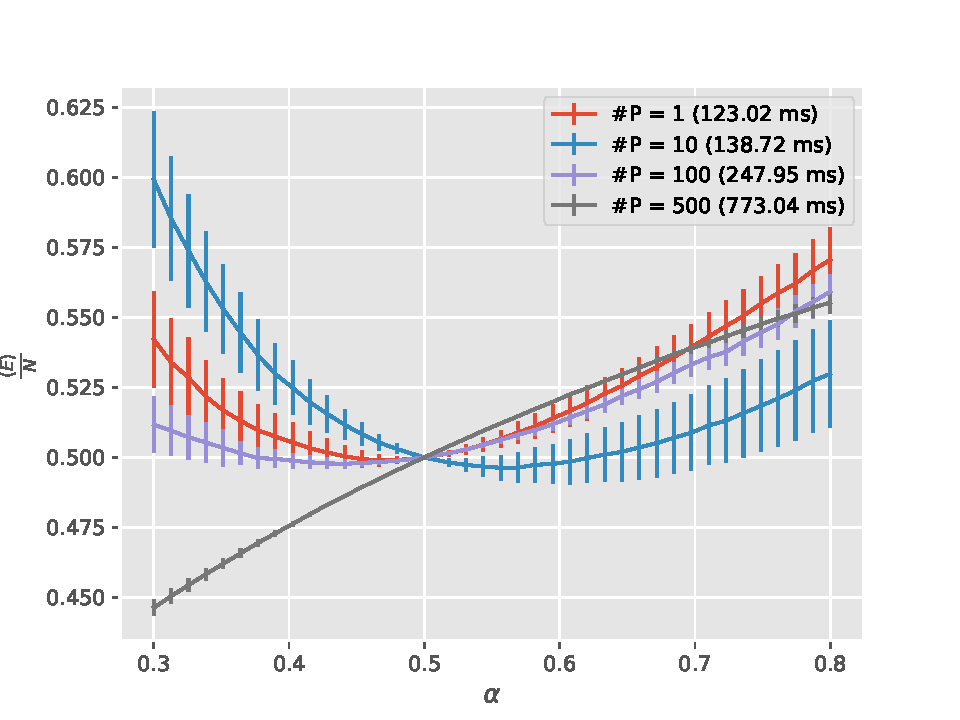
\includegraphics[trim=0cm 0.0cm 0cm 1.0cm, clip=true,scale = 0.7]{D_1_HarmonicOscillator SimpleGaussian Analytical_2pow18.pdf}
\caption[Insufficient equilibration steps]{The particle number- normalized expectation value for the energy as a function of the variational parameter $\alpha$.For 1 dimension, using $2^{18}$ MC- steps}\label{TooFew}
\end{figure}
We see that the systems with many particles no longer have a clear inflexion point at $\alpha = 0.5$. This is fixed by simply increasing the number of steps the algorithm runs before beginning sampling. As we see in figure \ref{Enough} below
\begin{figure}[H]
\centering

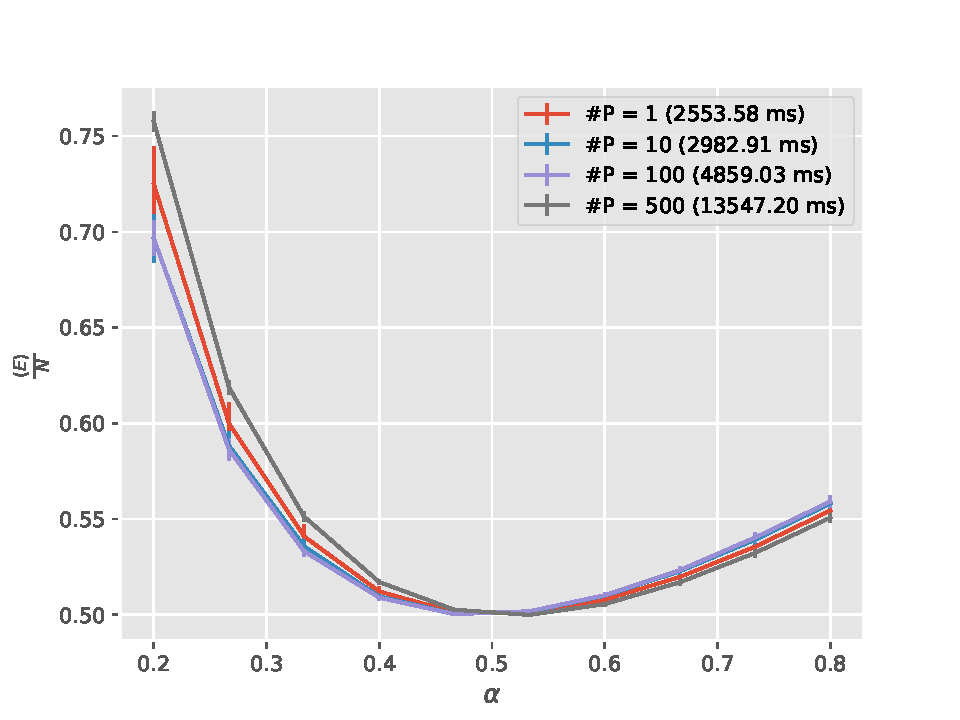
\includegraphics[trim=0cm 0.0cm 0cm 1.0cm, clip=true,scale = 0.7]{D_1_HarmonicOscillator_SimpleGaussian_Analytical_2pow22.pdf}
\caption[No interaction (1D)]{The particle number- normalized expectation value for the energy as a function of the variational parameter $\alpha$.For 1 dimension, using $2^{22}$ MC- steps}\label{Enough}
\end{figure}

we now have a clear inflexion point at $\alpha = 0.5$ with much smaller error bars. Additionally, the lines are much closer together, as they should be for an uncorrelated system. We also see that the lowest normalized energy is $0.5$. This is correct according to the analytical result for a 1- dimensional system with $\omega_{ho} = 1$ (see equation \eqref{eq:localEnergyAnalytical}).\\We have the same findings for the 2-, and 3- dimensional systems in figures \ref{2dUncorrolated} and \ref{3dUncorrolated} below.

\begin{figure}[H]
\centering

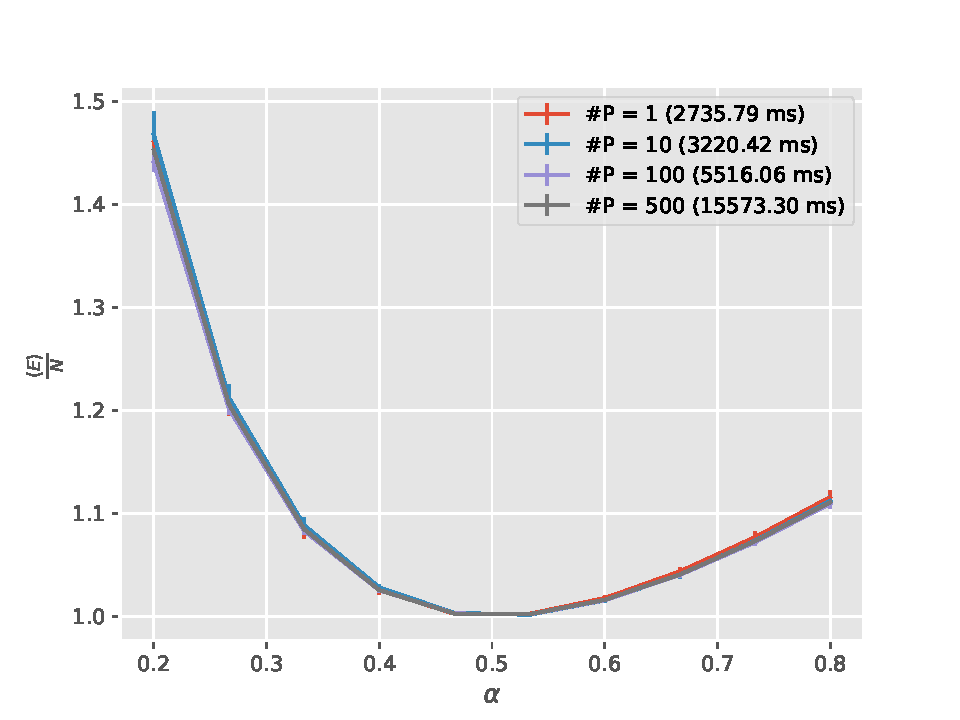
\includegraphics[trim=0cm 0.0cm 0cm 1.0cm, clip=true,scale = 0.7]{HarmonicOscillator_SimpleGaussian_D2_2pow22_analytic.pdf}
\caption[No interaction (2D)]{The particle number- normalized expectation value for the energy as a function of the variational parameter $\alpha$.For 2 dimensions, using $2^{22}$ MC- steps}\label{2dUncorrolated}
\end{figure}

\begin{figure}[H]
\centering

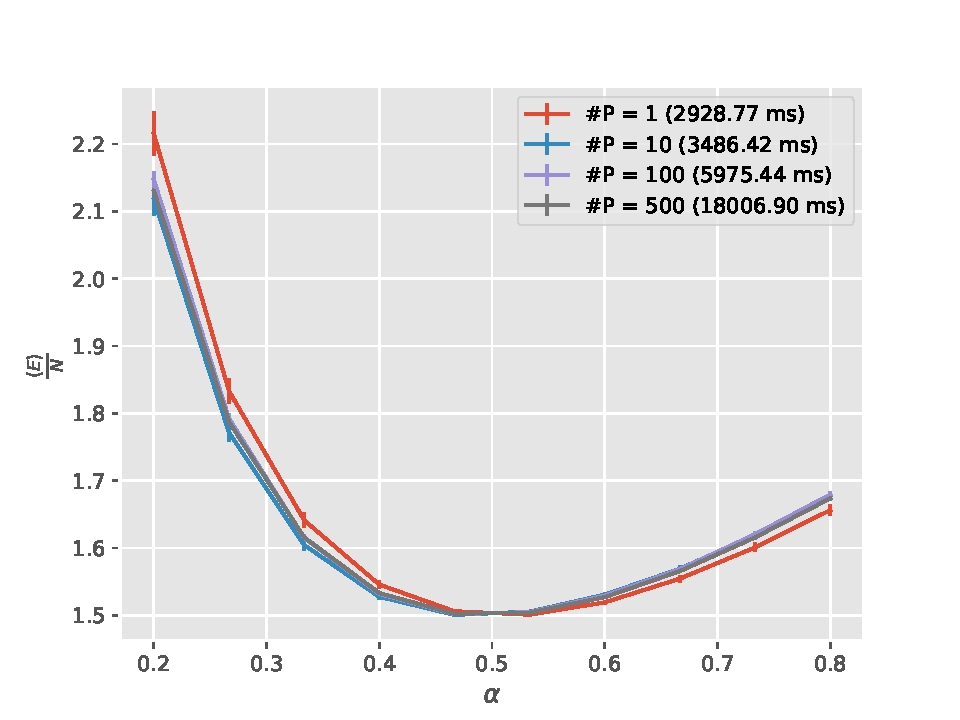
\includegraphics[trim=0cm 0.0cm 0cm 1.0cm, clip=true,scale = 0.7]{HarmonicOscillator_SimpleGaussian_D3_2pow22_analytic_NoTitle.pdf}
\caption[No interaction (3D)]{The particle number- normalized expectation value for the energy as a function of the variational parameter $\alpha$.For 3 dimensions, using $2^{22}$ MC- steps}\label{3dUncorrolated}
\end{figure}

\subsubsection{Analytic v. numerical derivative}
For the uncorrelated system, using the numerical double derivative for calculating the kinetic energy, we find that performing the same computation takes up to 115 times as long for 500 particles in 3 dimensions using $2^{22}$ steps.\\In figure \ref{1dNumeric} below, we see that the lowest normalized energy of $0.025$ happens at $\alpha = 0.6$ rather than $0.5$. This result is off by an order of magnitude.

\begin{figure}[H]
\centering

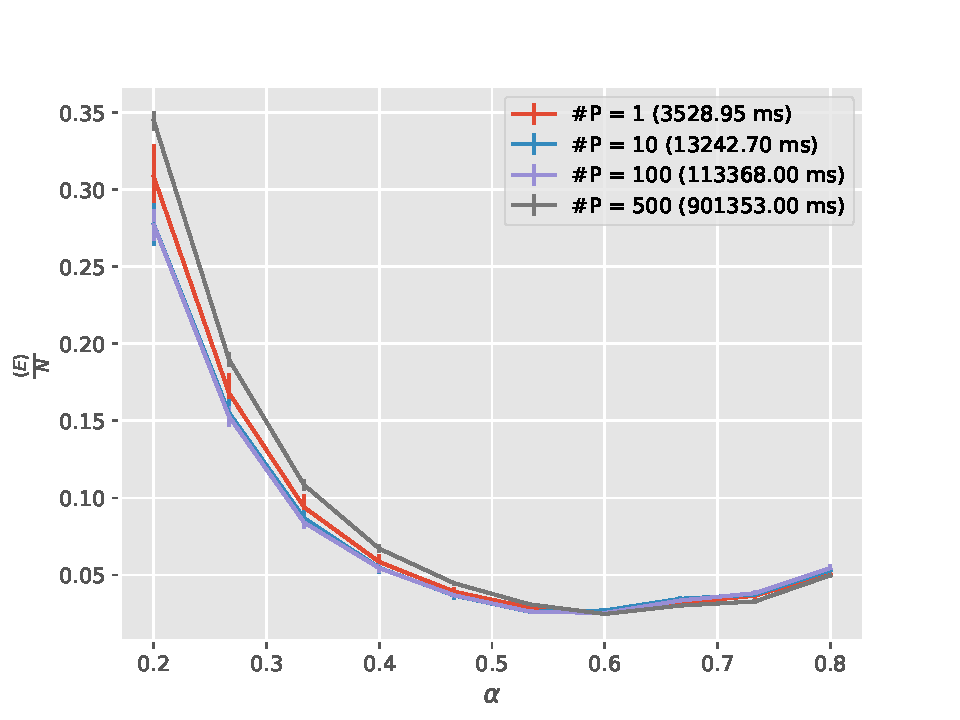
\includegraphics[trim=0cm 0.0cm 0cm 1.0cm, clip=true,scale = 0.7]{HarmonicOscillator_SimpleGaussianNumerical_D1_2pow22_numerical_NoTitle.pdf}
\caption[Numerical No interaction (1D)]{The particle number- normalized expectation value for the energy as a function of the variational parameter $\alpha$.For 1 dimension, using $2^{22}$ MC- steps and numerical differentiation}\label{1dNumeric}
\end{figure}

In figure \ref{2dNumeric} below, we again see that the energy is off by and order of magnitude while the energy minimum has shifted closer to $\alpha = 0.5$
\begin{figure}[H]
\centering

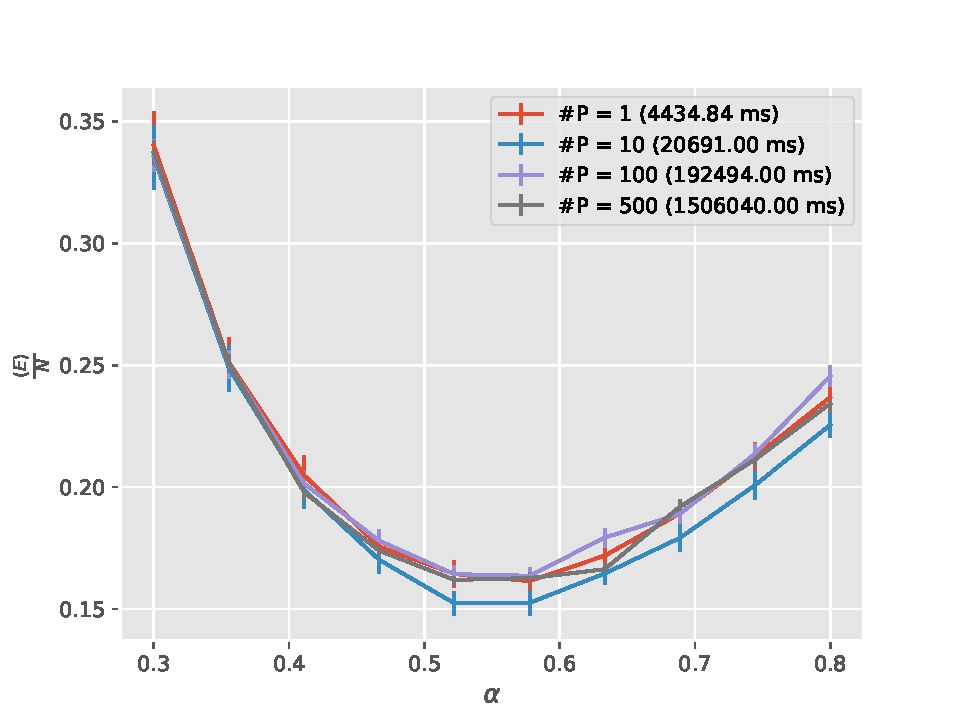
\includegraphics[trim=0cm 0.0cm 0cm 1.0cm, clip=true,scale = 0.7]{HarmonicOscillator_SimpleGaussianNumerical_D2_2pow22_numerical_NoTitle.pdf}
\caption[Numerical No interaction (2D)]{The particle number- normalized expectation value for the energy as a function of the variational parameter $\alpha$.For 2 dimensions, using $2^{22}$ MC- steps and numerical differentiation}\label{2dNumeric}
\end{figure}

In figure \ref{3dNumeric} below, we see that the energy is now only slightly off while the energy minimum is nearly happening at $\alpha = 0.5$ 

\begin{figure}[H]
\centering

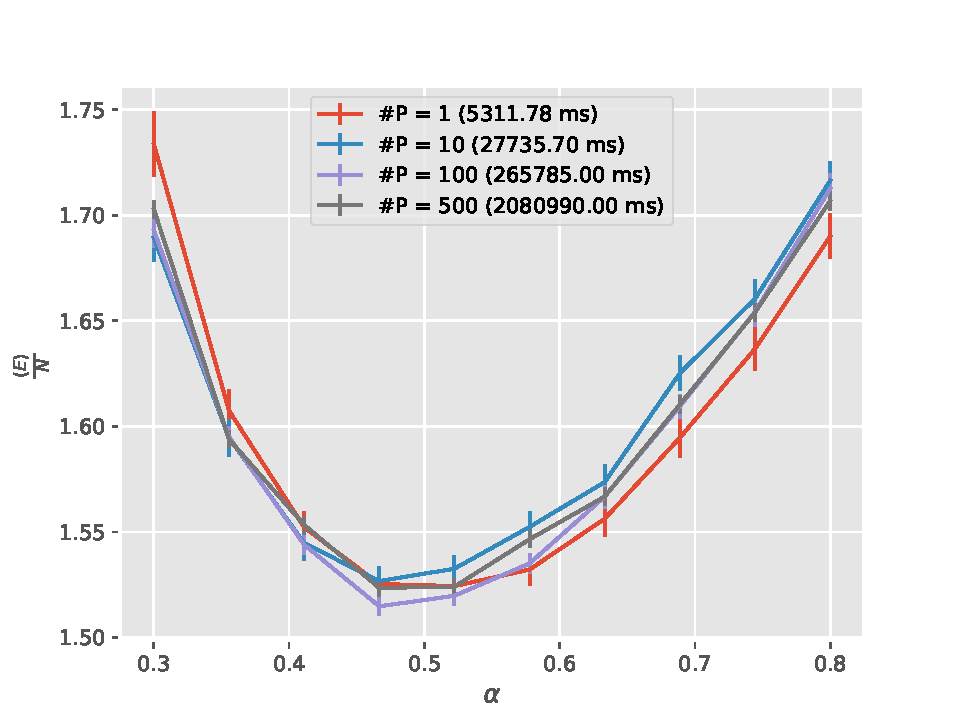
\includegraphics[trim=0cm 0.0cm 0cm 1.0cm, clip=true,scale = 0.7]{HarmonicOscillator_SimpleGaussianNumerical_D3_2pow22_numerical_NoTitle.pdf}
\caption[Numerical No interaction (3D)]{The particle number- normalized expectation value for the energy as a function of the variational parameter $\alpha$.For 3 dimensions, using $2^{22}$ MC- steps and numerical differentiation}\label{3dNumeric}
\end{figure}




\subsubsection{Importance  Sampling}
As we can see in figures \ref{imp1d},\ref{imp2d} and \ref{imp3d} below the addition of importance sampling on the uncorrelated systems gives the same minimums as brute force sampling, but the lines are now much closer together, indicating that the system has reached equilibration faster as they use the same number of Monte Carlo steps.

\begin{figure}[H]
\centering

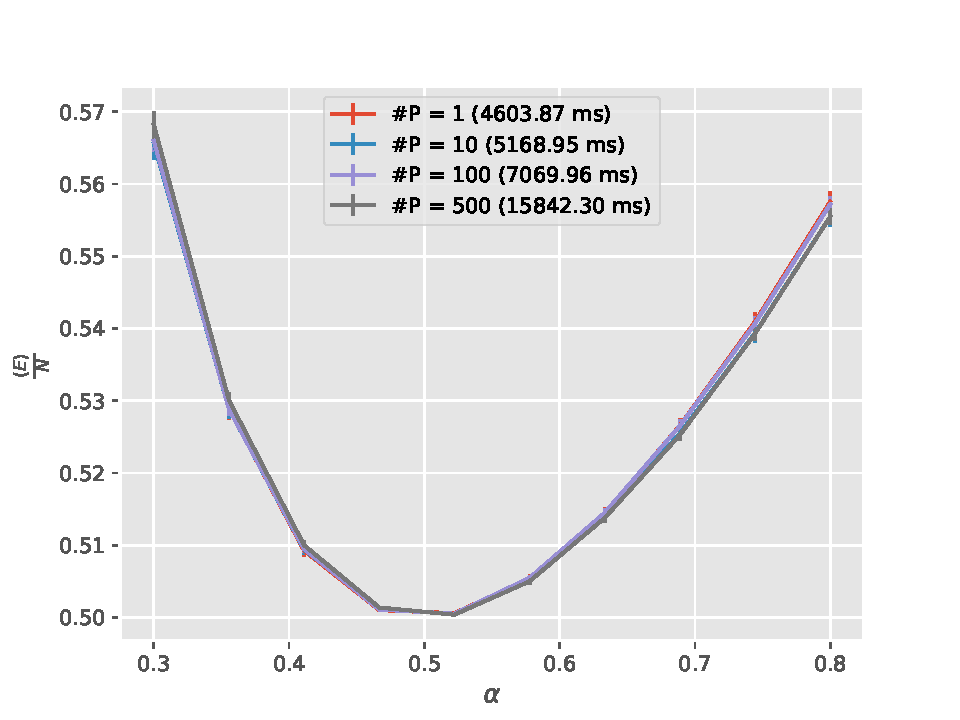
\includegraphics[trim=0cm 0.0cm 0cm 1.0cm, clip=true,scale = 0.7]{HarmonicOscillator_SimpleGaussian_D1_2pow22_task_C_1_NoTitle.pdf}
\caption[No interaction, importance sampling (1D)]{The particle number- normalized expectation value for the energy as a function of the variational parameter $\alpha$.For 1 dimension, using $2^{22}$ MC- steps  with importance sampling}\label{imp1d}
\end{figure}

\begin{figure}[H]
\centering

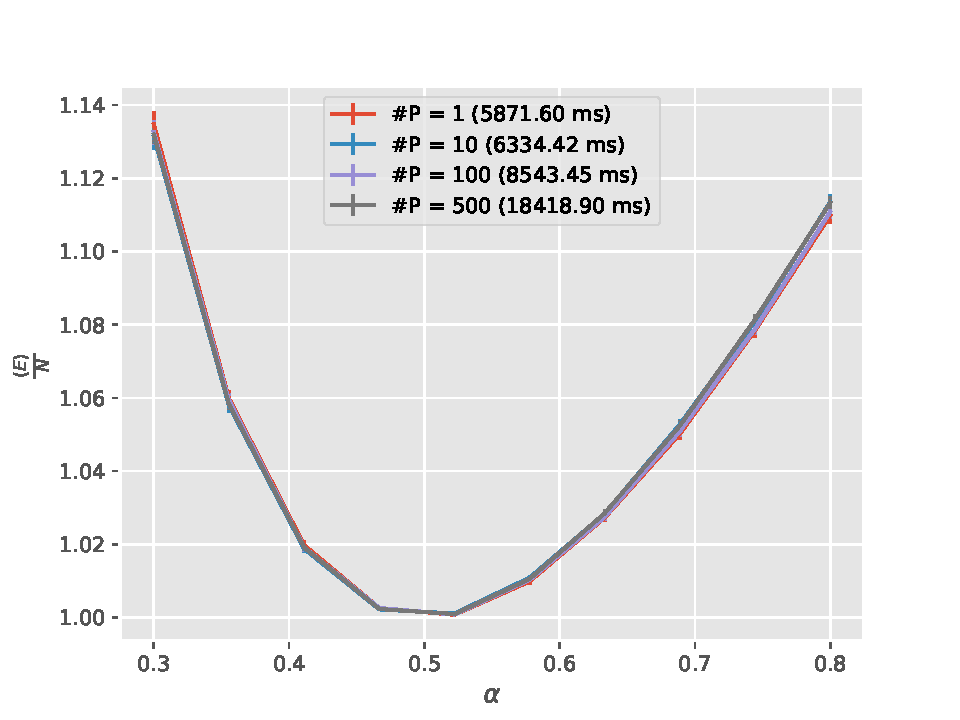
\includegraphics[trim=0cm 0.0cm 0cm 1.0cm, clip=true,scale = 0.7]{HarmonicOscillator_SimpleGaussian_D2_2pow22_task_C_1_NoTitle.pdf}
\caption[No interaction, importance sampling (2D)]{The particle number- normalized expectation value for the energy as a function of the variational paramter $\alpha$.For 2 dimensions, using $2^{22}$ MC- steps  with importance sampling}\label{imp2d}
\end{figure}

\begin{figure}[H]
\centering

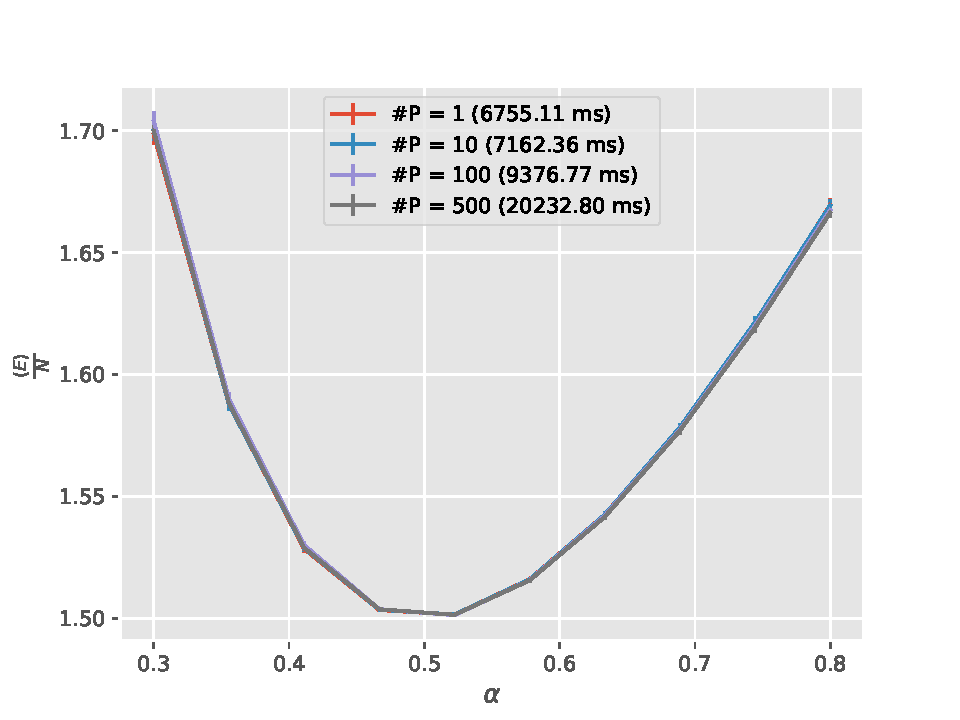
\includegraphics[trim=0cm 0.0cm 0cm 1.0cm, clip=true,scale = 0.7]{HarmonicOscillator_SimpleGaussian_D3_2pow22_task_C_1_NoTitle.pdf}
\caption[No interaction, importance sampling (3D)]{The particle number- normalized expectation value for the energy as a function of the variational parameter $\alpha$.For 3 dimensions, using $2^{22}$ MC- steps  with importance sampling}\label{imp3d}
\end{figure}

\subsubsection{Importance Sampling Time Step Dependence}
To study the effect of the time step $\delta t$ in equation \eqref{eq:Langevin_discrete}, we plot the proportion of the proposed steps that are accepted according to the Metropolis- Hastings algorithm as a function of the time step size. As we see in figure \ref{TimeStepDependence} below, the acceptance rate is highest for values closest to zero, with the smallest time step being $10^{-4}$. These small time steps come at the cost of slower equilibration as the particles take longer to travel. Clearly then, there is an optimal value for this time step as we want long enough to be efficient but also small enough to have a high acceptance rate. 
\begin{figure}[H]
\centering

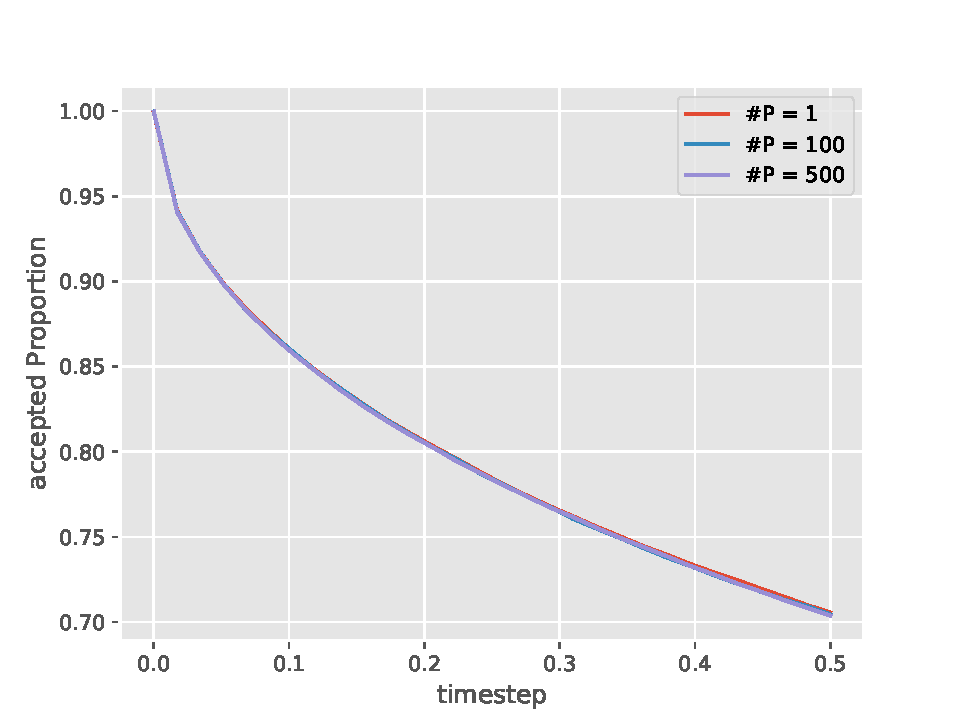
\includegraphics[trim=0cm 0.0cm 0cm 1.0cm, clip=true,scale = 0.7]{HarmonicOscillator_SimpleGaussian_D1_2pow18_task_C_2_NoTitle.pdf}
\caption[Importance sampling acceptance rate v time step]{The proportion of accepted moves as a function of the size of the time step. For 1 dimension, using $2^{18}$ MC- steps  with importance sampling}\label{TimeStepDependence}
\end{figure}


\subsection{Interacting particles in EHO}
For the interacting particles in the elliptical harmonic oscillator, we finally see that the normalized energies are diverging. As we can see, in figure \ref{interactElliptcEnergy} the normalized energy levels increase with increasing particle number. This is expected, as more particles interacting, will increase the energy.
\begin{figure}[H]
\centering

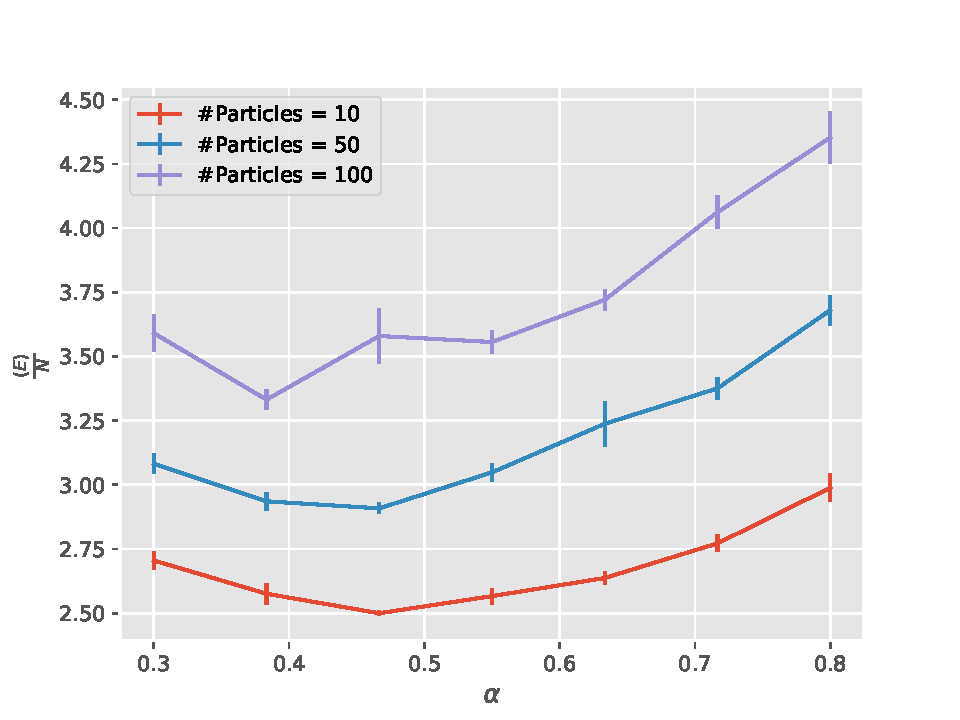
\includegraphics[trim=0cm 0.0cm 0cm 1.0cm, clip=true,scale = 0.7]{EllipticOscillator_CorrelatedGaussian_2pow18_NoTitle.pdf}
\caption[Interacting, EHO potential]{The particle number- normalized expectation value for the energy as a function of the variational parameter $\alpha$.For 3 dimensions, using $2^{18}$ MC- steps for the corrolated system in an elliptical HO- potential with $\gamma = \beta = 2.82843$.}\label{interactElliptcEnergy}
\end{figure}

\subsubsection{Steepest Descent Result}
Because large systems take so long to simulate, there hasn't been time to complete a gradient descent analysis for systems with 50 and 100 particles. Instead we have analyses for systems with 10, 20 and 30 particles to analyse how the values for the optimal $\alpha$ changes. Because we're searching the parameter space with a fixed step- size, we can provide an upper limit for the error in the optimal value for  $\alpha$.

\begin{table}[H]
\centering
\begin{tabular}{|l|l|l|}
\hline
Nr. Particles & $\braket{E}$       & $\alpha$               \\ \hline
10            & 25.3222 & $0.42 \pm 0.000909$      \\ \hline
20            & 53.8389 & $0.362182  \pm 0.00109$ \\ \hline
30            & 81.0876 & $0.402727 \pm 0.001363$    \\ \hline
\end{tabular}\caption[Optimal alpha from steepest descent]{Correlated EHO potential, upper bound for the error in provided by doing a grid search around $\alpha$ and seing that the energy increases in both directions.}\label{table}
\end{table}
Here we see the same trend that appeared in figure \ref{interactElliptcEnergy}, that the optimal value for $\alpha$ looks to shift towards a lower value, for systems with more particles.

\subsubsection{Time expenditure}
While the computation time in the non- interacting case has a nearly linear relationship with the number of particles, this is not the case in the case of interacting particles. We can see in figure \ref{InteractTimeExpend} a line of best fit through the time spent calculating a single data point for different numbers of particles. 
\begin{figure}[H]
\centering

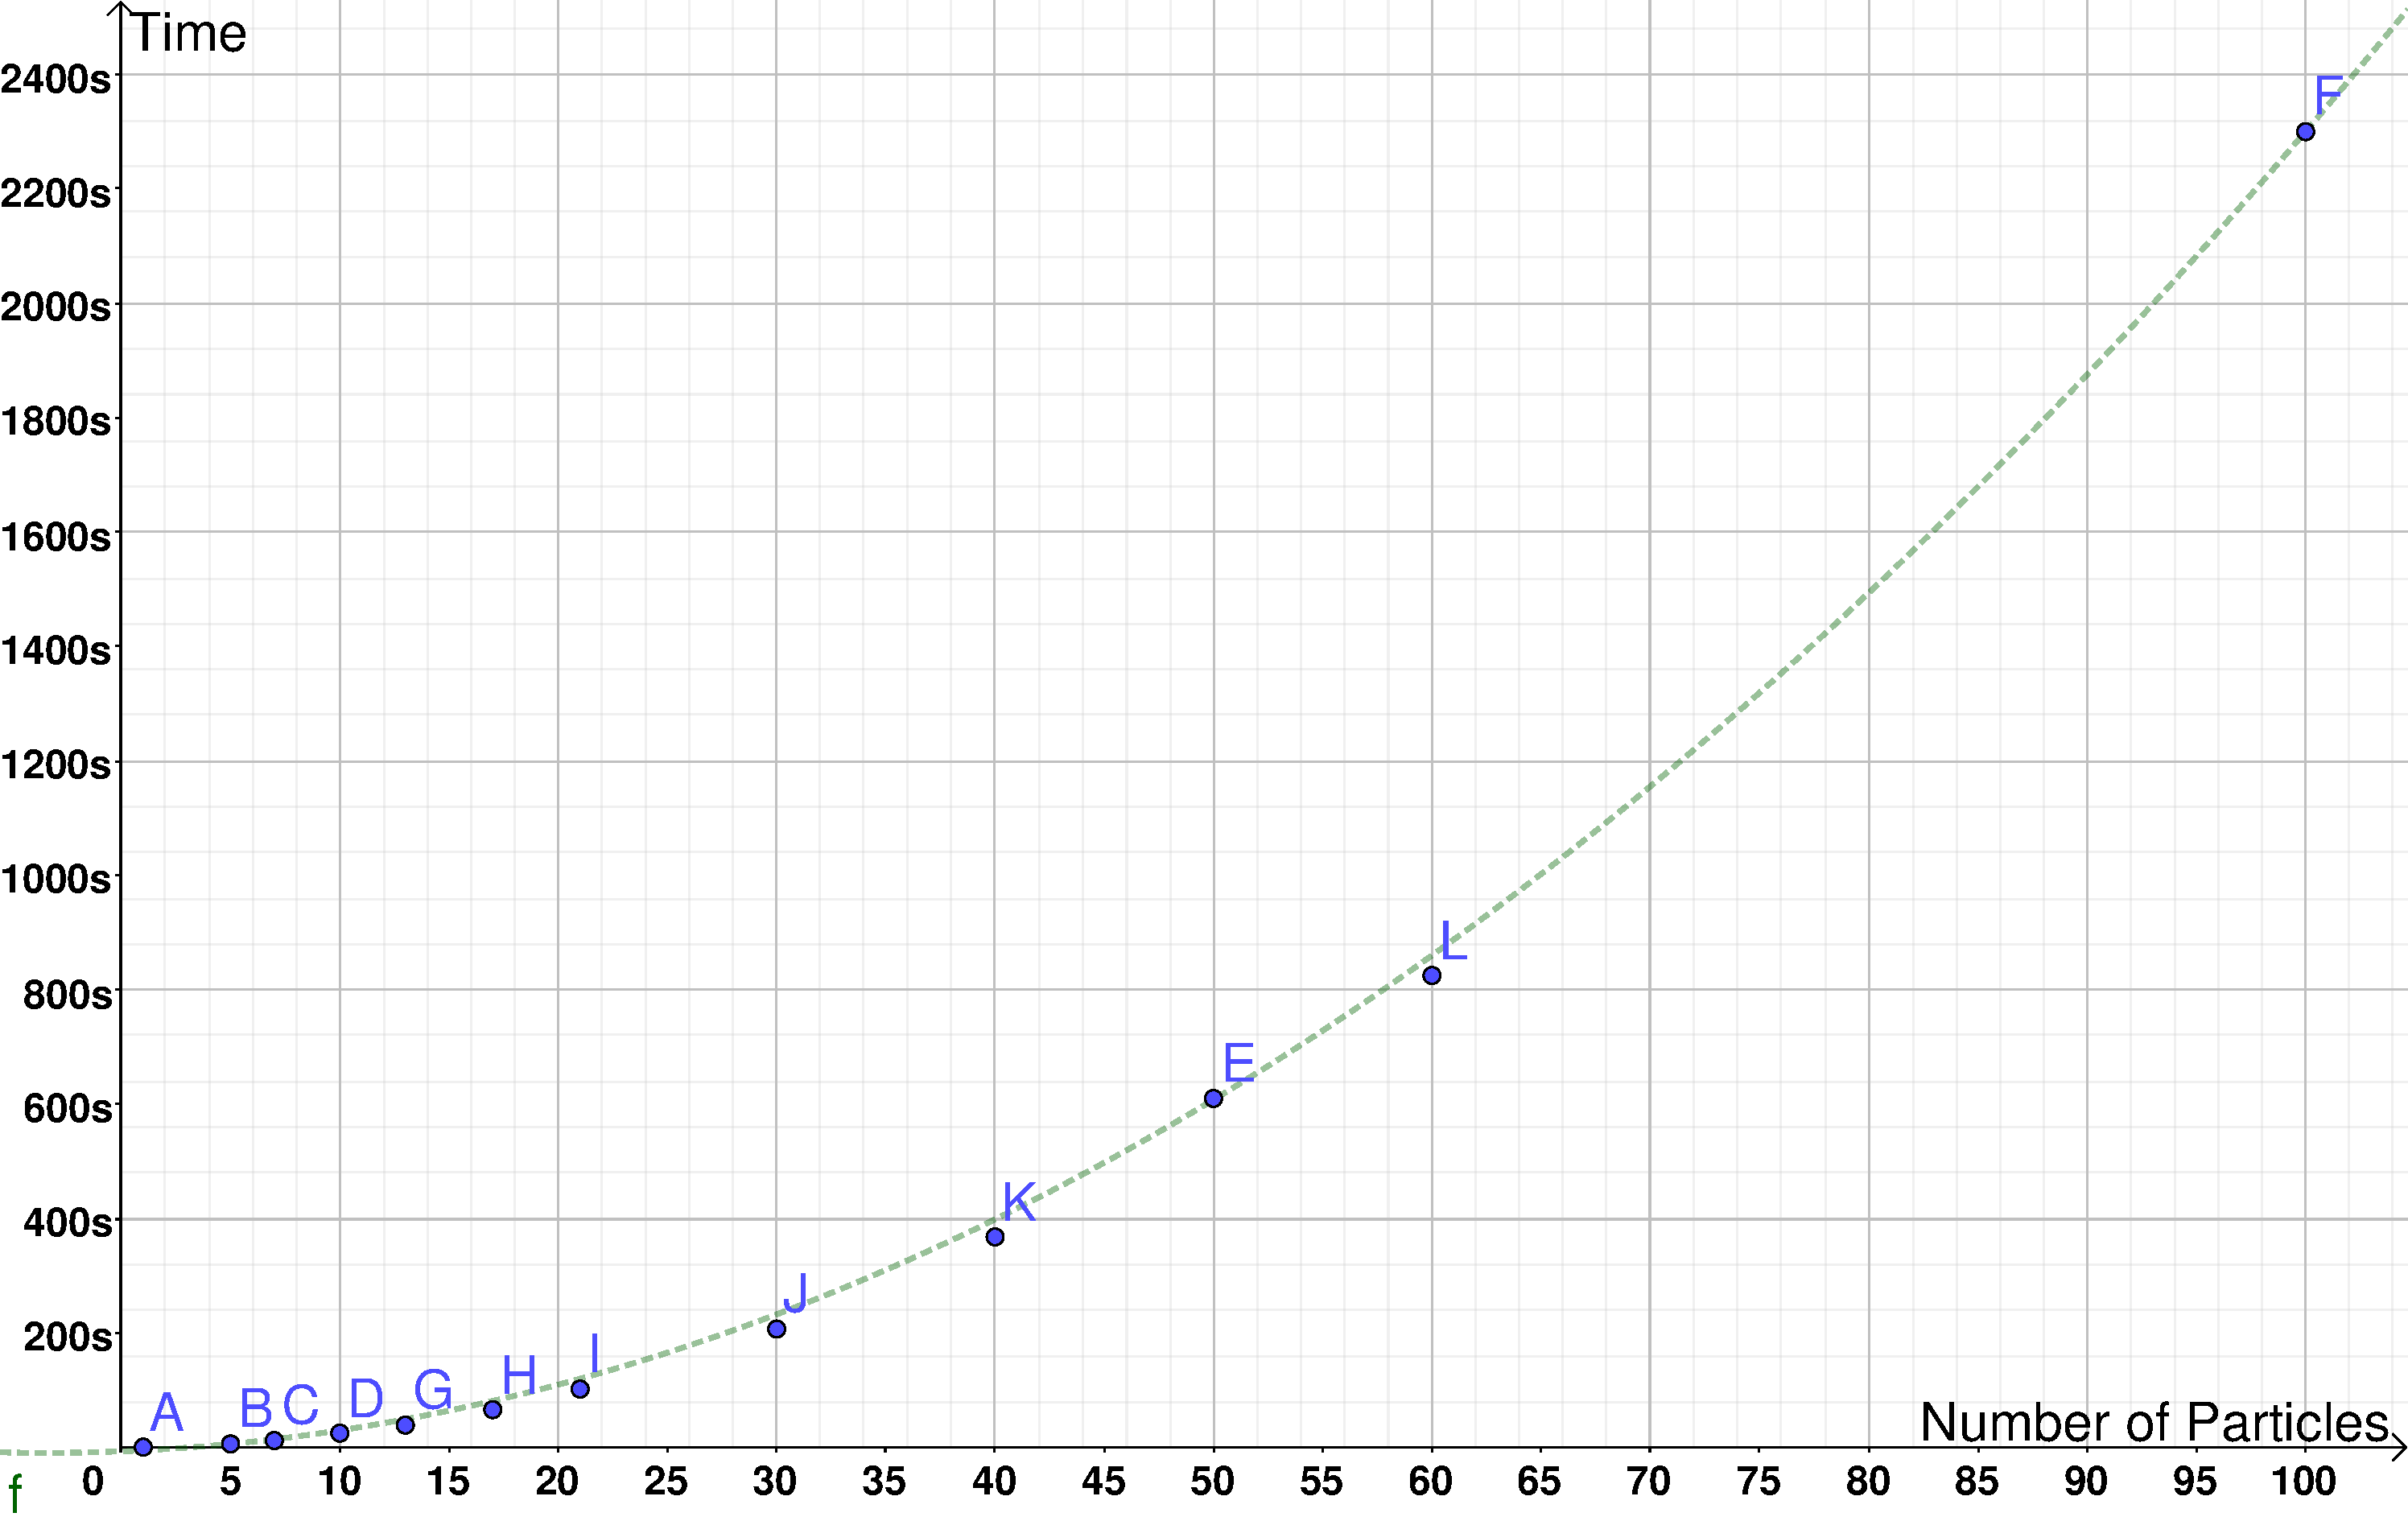
\includegraphics[trim=0cm 0.0cm 0cm 0.0cm, clip=true,scale = 0.25]{geogebra-export.pdf}
\caption[Time expended per datapoint (interacting) ]{Time expenditure per datapoint in seconds v. the number of particles for a correlated system with an elliptical HO- potential using $2^{18}$ MC- steps.}\label{InteractTimeExpend}
\end{figure}
the relationship turns out to be a 2'nd degree polynomial. 
\subsection{The Jastrow factor and The Distribution of Bosons}
By changing the so- called Hard- Core Diameter of the bosons, we can influence the Jastrow factor and study its effects. We see the results of this in figure \ref{fig:Jastrows} below.

\begin{figure}[H]

\centering

\begin{subfigure}{.5\textwidth}
  \centering
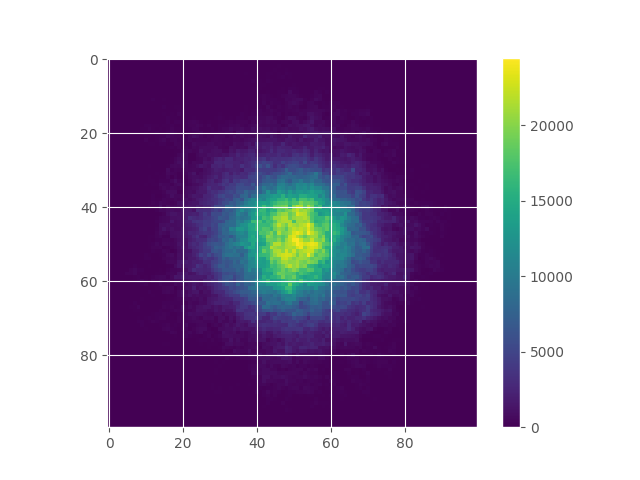
\includegraphics[trim=3cm 0.0cm 1.5cm 0.0cm, clip=true,scale = 0.45]{NoJastrow_20.png}
\caption{Hard- Core diameter $= 0$}\label{J1}
\end{subfigure}%
\begin{subfigure}{.5\textwidth}
  \centering
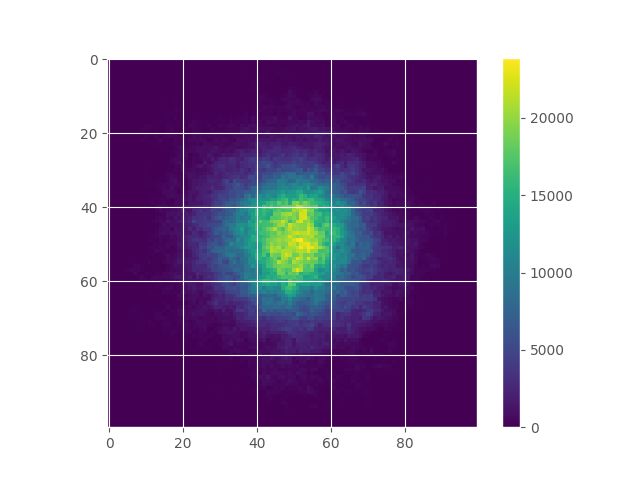
\includegraphics[trim=3cm 0.0cm 1.5cm 0.0cm, clip=true,scale = 0.45]{Jastrow_20.png}
\caption{Hard- Core diameter $= 0.00433$}\label{J2}
\end{subfigure}
\begin{subfigure}{.5\textwidth}
  \centering
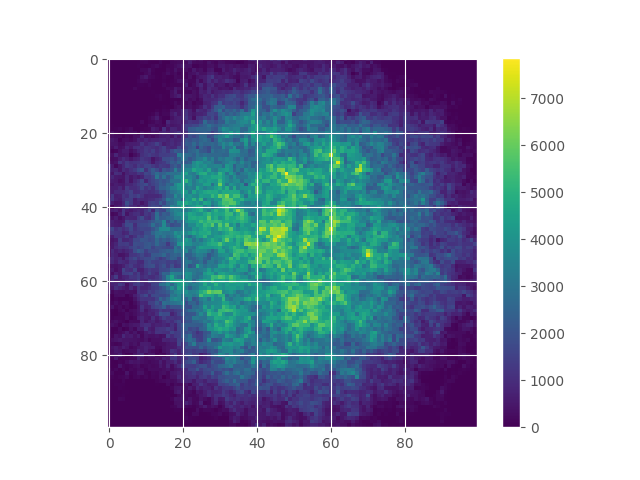
\includegraphics[trim=3cm 0.0cm 1.5cm 0.0cm, clip=true,scale = 0.45]{LargeJastrow_20.png}
\caption{Hard- Core diameter $= 0.433$}\label{J3}
\end{subfigure}%
\begin{subfigure}{.5\textwidth}
  \centering
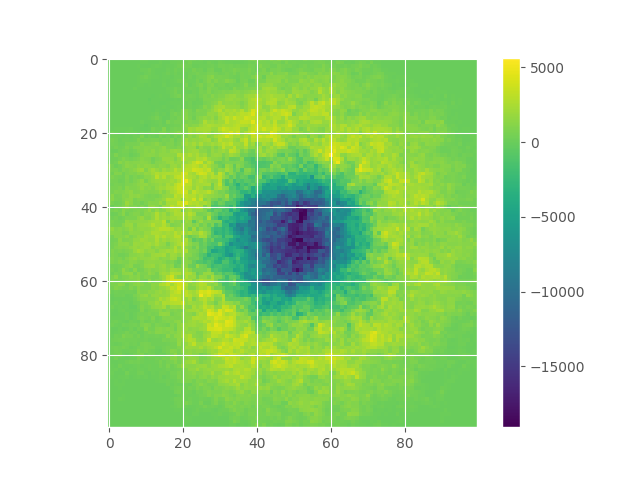
\includegraphics[trim=3cm 0.0cm 1.5cm 0.0cm, clip=true,scale = 0.45]{LargeJastrow_minus_Jastrow_20.png}
\caption{Figure \ref{J3} minus Figure \ref{J2}}\label{J4}
\end{subfigure}

\caption[Effect of the Jastrow factor on the XY- distribution of bosons]{The distribution of bosons projected onto the xy- plane using 20 particles in three dimensions, $\alpha = 0.5$ and $2^{20}$ Monte- Carlo steps. The Hard- Core Diameter is $0.00433$ as per \cite{DuBois_2001} and \cite{Nilsen_2005}. Each grid- line corresponds to $1.2$ units of distance.}.
\label{fig:Jastrows}
\end{figure}

As we can see, between figures \ref{J1} and \ref{J2} the difference is nearly imperceptible, with only a slight dimming of the central spot. The difference becomes much more noticeable between figures \ref{J2} and \ref{J3} with their difference shown in figure \ref{J4}. The bosons become much more spread out, as clustering together takes more energy when the Jastrow factor is higher. In order to see the difference between The system with and without the Jastrow factor, we have too look at systems with more particles. In figure \ref{150Particles_Jastrow_minus_NoJastrow} below, we see the difference in the number of particles sampled in each colored square (Jastrow factor minus no Jastrow factor). We see clearly that particles are migrating to occupy a greater area. This effect is much more noticeable with 150 particles rather than the 20 used in figure \ref{fig:Jastrows}.

\begin{figure}[H]
\centering

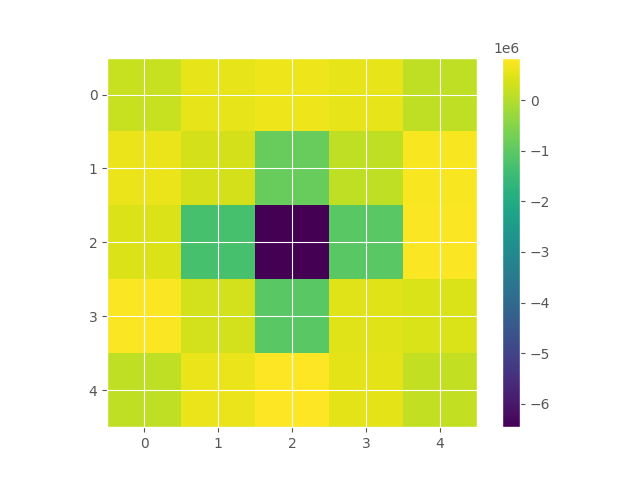
\includegraphics[trim=0cm 0.0cm 0cm 0.0cm, clip=true,scale = 0.5]{Jastrow_minus_NoJastrow_150.png}
\caption[]{The distribution of bosons projected onto the xy- plane using 150 particles in three dimensions, $\alpha = 0.5$ and $2^{20}$ Monte- Carlo steps. This is the result of subtracting the data using a Hard- Core Diameter is $0.00433$ as per \cite{DuBois_2001} and \cite{Nilsen_2005} by the data from no Jastrow factor.}\label{150Particles_Jastrow_minus_NoJastrow}
\end{figure}



\section{Conclusion}
Based on the success of the program in the non- interacting case we can conclude that both the Metropolis Algorithm and The Metropolis- Hastings algorithm were correctly implemented. The implementation of numerical differentiation had unstable results when varying the step length and there wasn't enough time to find an optimal step length for the different systems. This implementation was largely a failure, as it yielded results that were wrong by an order of magnitude. The difference in time- expenditure was substantial, proving that analytical solutions should be applied where possible.\\\\We saw that importance sampling greatly contributed in reducing the error in the energy calculation, as the system equilibrated earlier.\\The implementation of the full correlated system in the elliptical harmonic oscillator showed that there is an additional gain in energy with more particles beyond the the simple multiplicative factor coming from multiplying the one- body problem. The optimal value for $\alpha$ seemed to shift to lower values in the systems with the most particles.\\\\There are several things that should be implemented and improved upon. The number of equilibration steps should not be decided by some arbitrary number. We could instead sample a running mean and start sampling only when the variance falls below a desired value, then sample for some number of steps that are a multiple of two, so as to work with Blocking. The Energies obtained through gradient descent, need error estimates but again, there wasn't time. \\ With a way to classify the end of equilibration, we could study the time to reach equilibration v. the length of the time step in order to obtain an optimal value for the time step, as it's a trade- off between the acceptance rate and the time taken to reach equilibration.\\\\More of the code should have been optimized for parallelization, as currently there are a lot of dependencies between classes that prohibit the compiler from vectorizing and parallelizing the code.

\section{Appendix A}\label{app_A}
We rewrite 
\begin{equation*}
\Psi_T(\mathbf{r})=\Psi_T(\mathbf{r}_1, \mathbf{r}_2, \dots \mathbf{r}_N,\alpha,\beta)
=\left[
    \prod_i g(\alpha,\beta,\mathbf{r}_i)
\right]
\left[
    \prod_{j<k}f(a,|\mathbf{r}_j-\mathbf{r}_k|)
\right],
\end{equation*}
as

\begin{equation*}
\Psi_T(\mathbf{r})=\left[
    \prod_i g(\alpha,\beta,\mathbf{r}_i)
\right]
\exp{\left(\sum_{j<k}u(r_{jk})\right)}
\end{equation*}
where we have defined $r_{ij}=|\mathbf{r}_i-\mathbf{r}_j|$
and

\begin{equation*}
   f(r_{ij})= \exp{\left(u(r_{ij})\right)},
\end{equation*}
with $u(r_{ij})=\ln{f(r_{ij})}$.
We also write

\begin{equation*}
    g(\alpha,\beta,\mathbf{r}_i) = \exp{\left[-\alpha(x_i^2+y_i^2+\beta
    z_i^2)\right]}= \phi(\mathbf{r}_i).
\end{equation*}
Starting with the gradient, we get
\begin{equation}
  \nabla_k\Psi_T(\mathbf{r}) = \exp{\left(\sum_{j<m}u(r_{jm})\right)}\nabla_k\left[\prod_{i}\phi(\mathbf{r}_i)\right] + \left[\prod_{i}\phi(\mathbf{r}_i)\right]\nabla_k\exp{\left(\sum_{j<m}u(r_{jm})\right)}
\end{equation}
solving each gradient separately, we get
\begin{equation*}
\nabla_k\left[\prod_{i}\phi(\mathbf{r}_i)\right] = \nabla_k\phi(\mathbf{r}_k)\left[\prod_{i\ne k}\phi(\mathbf{r}_i)\right]
\end{equation*}
and 
\begin{equation*}
\nabla_k\exp{\left(\sum_{i<k}u(r_{ik})\right)} = \exp{\left(\sum_{j<m}u(r_{jm})\right)}\sum_{l\ne k}\nabla_k u(r_{kl})
\end{equation*}
giving us 
\begin{align*}
  \nabla_k\Psi_T(\mathbf{r}) &= \nabla_k\phi(\mathbf{r}_k)\left[\prod_{i\ne k}\phi(\mathbf{r}_i)\right]\exp{\left(\sum_{j<m}u(r_{jm})\right)}
  \\
  &\qquad
  +  \left[\prod_i\phi(\mathbf{r}_i)\right]
  \exp{\left(\sum_{j<m}u(r_{jm})\right)}\sum_{l\ne k}\nabla_k u(r_{kl}),
\end{align*}
From here, we need to find the Laplacian. We accomplish this by taking the scalar product of the gradient we just got, with the gradient operator. Solving each term in turn, we get
\begin{equation*}
\left[\prod_{i\ne k}\phi(\mathbf{r}_i)\right]\left( \nabla_k^2\phi(\mathbf{r}_k) \exp{\left(\sum_{j<m}u(r_{jm})\right)} + \nabla_k\phi(\mathbf{r}_k)\nabla_k\exp{\left(\sum_{j<m}u(r_{jm})\right)}\right)
\end{equation*}
\begin{equation*}
= \left[\prod_{i\ne k}\phi(\mathbf{r}_i)\right]\exp{\left(\sum_{j<m}u(r_{jm})\right)}\left( \nabla_k^2\phi(\mathbf{r}_k)  + \nabla_k\phi(\mathbf{r}_k)\left(\sum_{j\ne k}\frac{(\mathbf{r}_k-\mathbf{r}_j)}{r_{kj}}u'(r_{kj})\right)\right)
\end{equation*}
and for the second term, 
\begin{equation*}
\nabla_k\phi(\mathbf{r}_k)\left[\prod_{i\ne k}\phi(\mathbf{r}_i)\right]\exp{\left(\sum_{j<m}u(r_{jm})\right)}\sum_{l\ne k}\nabla_k u(r_{kl}) + 
\end{equation*}
\begin{equation*}
\left[\prod_{i}\phi(\mathbf{r}_i)\right]\exp{\left(\sum_{j<m}u(r_{jm})\right)}\left(\sum_{j\ne k}\frac{(\mathbf{r}_k-\mathbf{r}_j)}{r_{kj}}u'(r_{kj})\right)\sum_{l\ne k}\nabla_k u(r_{kl}) + 
\end{equation*}
\begin{equation*}
\left[\prod_i\phi(\mathbf{r}_i)\right]
  \exp{\left(\sum_{j<m}u(r_{jm})\right)}\nabla_k\sum_{l\ne k}\nabla_k u(r_{kl}).
\end{equation*}
We can now resolve the last of the gradients while dividing every term by the trial wave function, this in turn, gets us the final expression for the normalized Laplacian of the trial wave function

\begin{align}
   \frac{1}{\Psi_T(\mathbf{r})}\nabla_k^2\Psi_T(\mathbf{r})
   &= \frac{\nabla_k^2\phi(\mathbf{r}_k)}{\phi(\mathbf{r}_k)}
   + 2\frac{\nabla_k\phi(\mathbf{r}_k)}{\phi(\mathbf{r}_k)}
   \left(\sum_{j\ne k}\frac{(\mathbf{r}_k-\mathbf{r}_j)}{r_{kj}}u'(r_{kj})\right)
   \\
   &\qquad
   + \sum_{i\ne k}\sum_{j \ne k}\frac{(\mathbf{r}_k-\mathbf{r}_i)(\mathbf{r}_k-\mathbf{r}_j)}{r_{ki}r_{kj}}u'(r_{ki})u'(r_{kj})
   \\
   &\qquad
   + \sum_{j\ne k}\left( u''(r_{kj})+\frac{2}{r_{kj}}u'(r_{kj})\right).
\end{align}
\bibliographystyle{plain}
\bibliography{references}
\end{document}
